% -*- TeX:de -*-
\NeedsTeXFormat{LaTeX2e}
\documentclass[12pt,a4paper,titlepage]{article}

%\usepackage[german]{babel} % german text
\usepackage[DIV12]{typearea} % size of printable area
\usepackage[T1]{fontenc} % font encoding
\usepackage[utf8]{inputenc} % probably on Linux

\usepackage{graphicx} % to include images
\usepackage{subfigure} % for creating subfigures
\usepackage{amsmath} % a bunch of symbols
\usepackage{amssymb} % even more symbols
\usepackage{booktabs} % pretty tables
\usepackage{csquotes}

% a floating environment for circuits
\usepackage{float}
\usepackage{caption}

\newfloat{circuit}{tbph}{circuits}
\floatname{circuit}{Schaltplan}

% a floating environment for diagrams
\newfloat{diagram}{tbph}{diagrams}
\floatname{diagram}{Diagramm}

\renewcommand{\familydefault}{\sfdefault} % activate to use sans-serif font as default

\sloppy % friendly typesetting

\usepackage{eurosym}
\usepackage{makeidx}
\usepackage{amsfonts}
\usepackage{mparhack}
\usepackage{array}
\usepackage{tabularx}
\usepackage{minitoc}
\usepackage[colorlinks=true]{hyperref}
\usepackage{epstopdf}
\usepackage{setspace}
\usepackage{csquotes}

\begin{document}

\begin{titlepage}

\begin{figure*}[h!]
  
\includegraphics[width=8cm]{TULogo_CMYK}
\end{figure*}

\begin{center}
\vspace*{1.3cm}
{\Huge Elektrotechnische Grundlagen der Informatik\\(LU 182.692)\\}
\vspace{1.7cm}
{\LARGE Protokoll der 2. Laborübung: \enquote{Filter}\\}
{\large \enquote{Transiente Vorgänge und Frequenzverhalten}\\}
{\LARGE a) LTSPICE-Simulationen\\}
\vspace{1.5cm}

% fill in group number and date of lab here
% CHANGE ME!
{\Large Gruppennr.: \ldots \hspace{1cm} Datum der Laborübung: \ldots\ldots\ldots\ldots\ldots}

% fill in IDs and names here
% CHANGE ME!
\begin{table}[h!]
\centering
\begin{tabular}{|p{3.5cm}|p{3.5cm}|p{6.5cm}|}
\hline \textbf{Matr. Nr.} & \textbf{Kennzahl} & \textbf{Name} \\
\hline
& & \\
\hline
& & \\
\hline
& & \\
\hline
\end{tabular}
\end{table}

\end{center}
\vspace{1.0cm}

\begin{table}[h!]
\begin{tabular}{|l|l|}
\hline \textbf{Kontrolle} & \checkmark \\
\hline Verhalten eines Filters 1. Ordnung & \\
\hline Verhalten eines RL-Filters & \\
\hline Dynamisches System 2. Ordnung & \\
\hline
\end{tabular}
\end{table}

\end{titlepage}
\setcounter{page}{2}

% start of actual lab protocol
% CHANGE ME!

\section{RC-Tiefpassilter 1. Ordnung}

\subsection{Aufgabenstellung}
Die Sprungantwort und der Amplituden- bzw. Phasengang eines RC-Tiefpassilters 1. Ordnung soll mittels LTSpice simuliert werden.

\subsection{Schaltplan}

\begin{figure}[H]
  \centering
  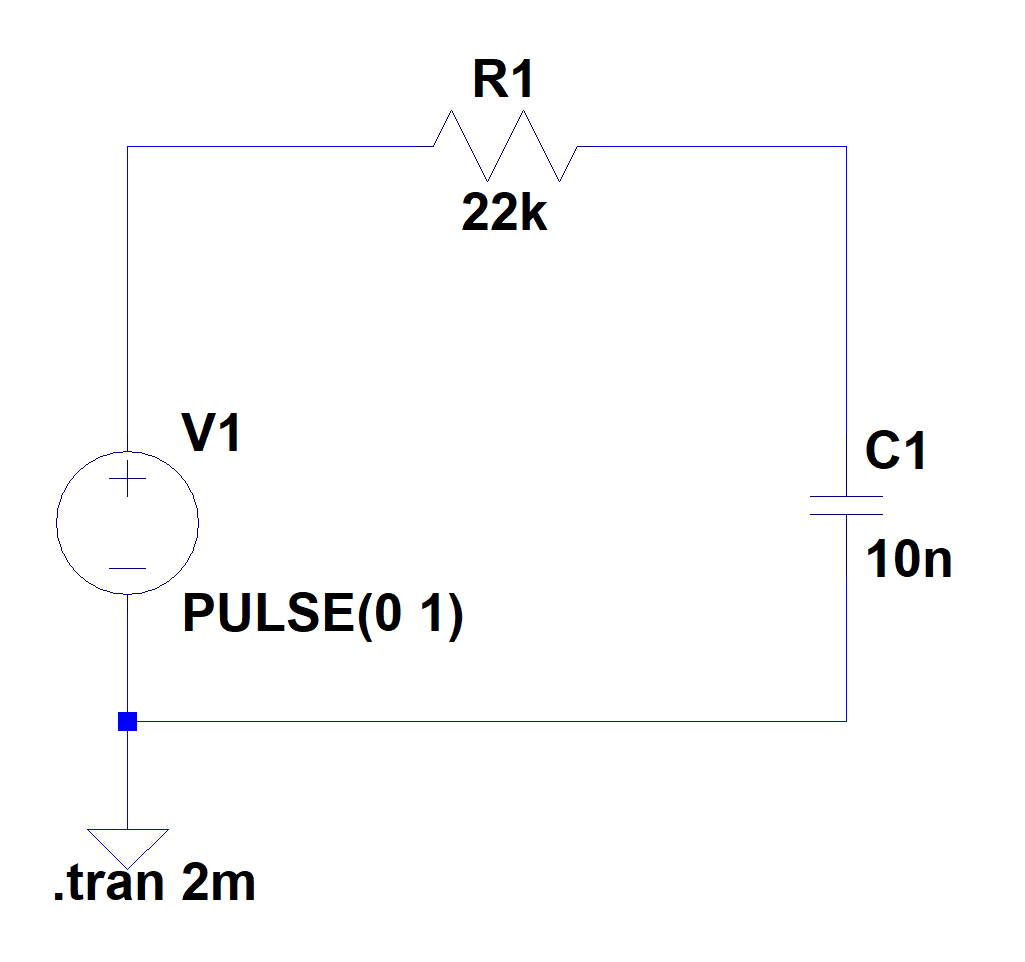
\includegraphics[width=100mm]{filter01_schaltung.PNG}
  \caption{RC-Tiefpassfilter 1. Ordnung}
\end{figure}

\subsection{Durchführung}
Zuerst wird die RC-Schaltung mit $R1 = 22k\Omega$ und $C1 = 10nF$ zusammengefügt. Dazu wird mit der PULSE-Option der Sprung von $0V$ auf $1V$ angelegt. Die Sprungantwort des Systems wird dann im Bereich von $0s$ bis $2ms$ geplotted. Nun soll der Amplituden- und Phasengang simuliert werden. Dazu wird eine sinusförmige Spannung mit $1V_{pp}$ ($0,5V$ Amplitude) angelegt. Es wird eine dekadische Simulation im Bereich von $1Hz$ bis $1MHz$ durchgeführt und das daraus resultierende Bode-Diagramm aufgezeichnet.

\subsection{Ergebnis}

\begin{figure}[H]
  \centering
  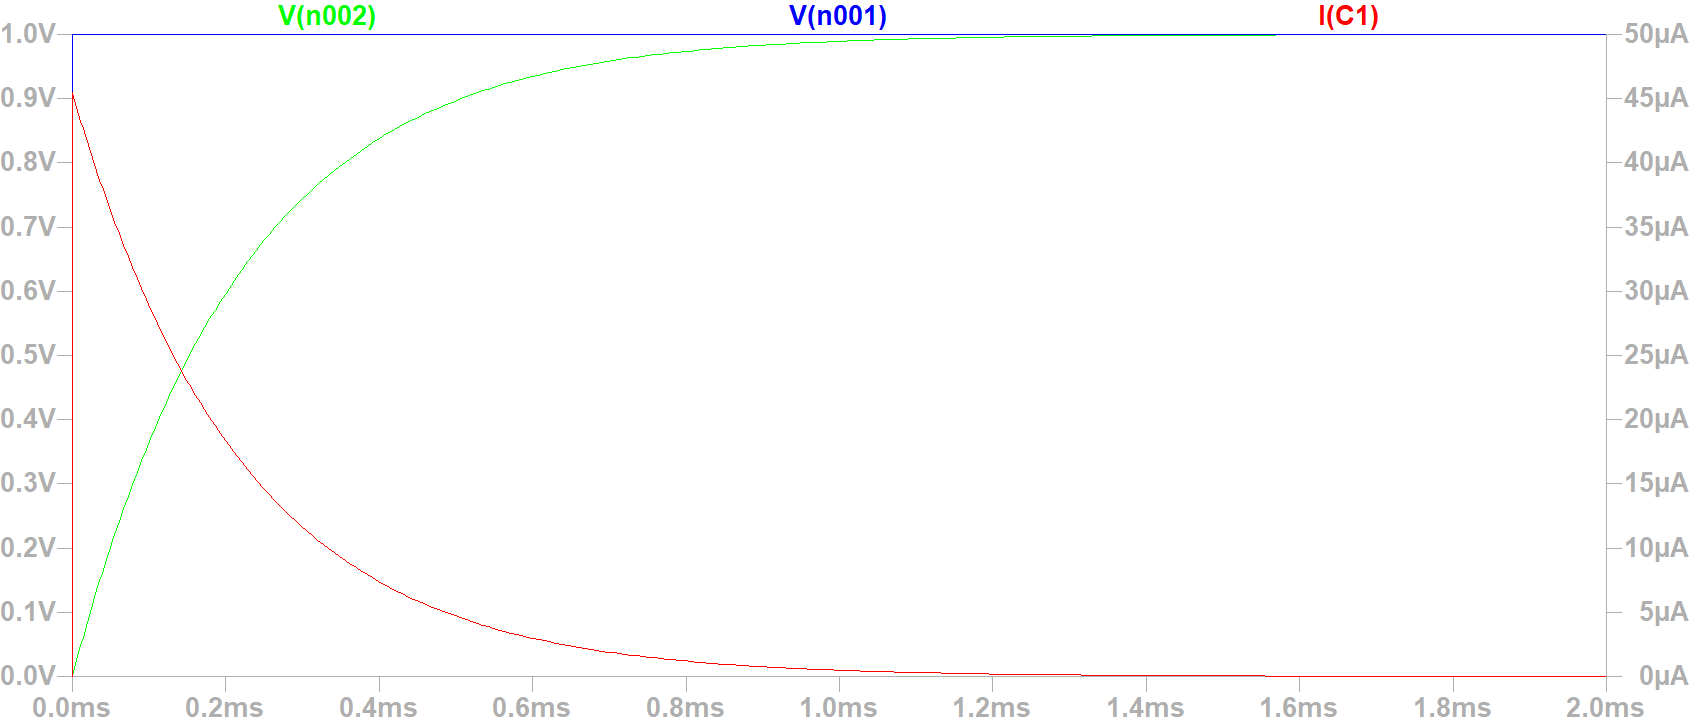
\includegraphics[width=150mm]{sprungantwort_filter01.png}
  \caption{Sprungantwort RC-Tiefpassfilter 1. Ordnung}
\end{figure}

Anhand dieses Diagramms erkennt man sehr gut, wie der Strom $I(C1)$ am Kondensator zuerst maximal ist und bei steigender Spannung $V(n002)$ am Kondensator immer stärker abfällt. Der Strom erreicht seinen Tiefpunkt, sobald die Spannung am Kondensator maximal ist.\\\\
Die Zeitkonstante
\begin{figure}[H]
  \centering
  $\tau = R1*C1 = 22k\Omega*10nF = 220\mu s$
\end{figure}
\noindent besagt, dass nach $222\mu s$ 63\% der Maximalspannung von $C1$ erreicht wird. Dies lässt sich gut am Diagramm ablesen, wo die Spannung $V(n002)$ bei $0,22ms$ ca. $0,63V$ beträgt. Nach $5*\tau = 1,1ms$ wird 99\% der Maximalspannung erreicht, der Kondensator ist de facto vollständig geladen, die Spannung ist maximal.

\begin{figure}[H]
  \centering
  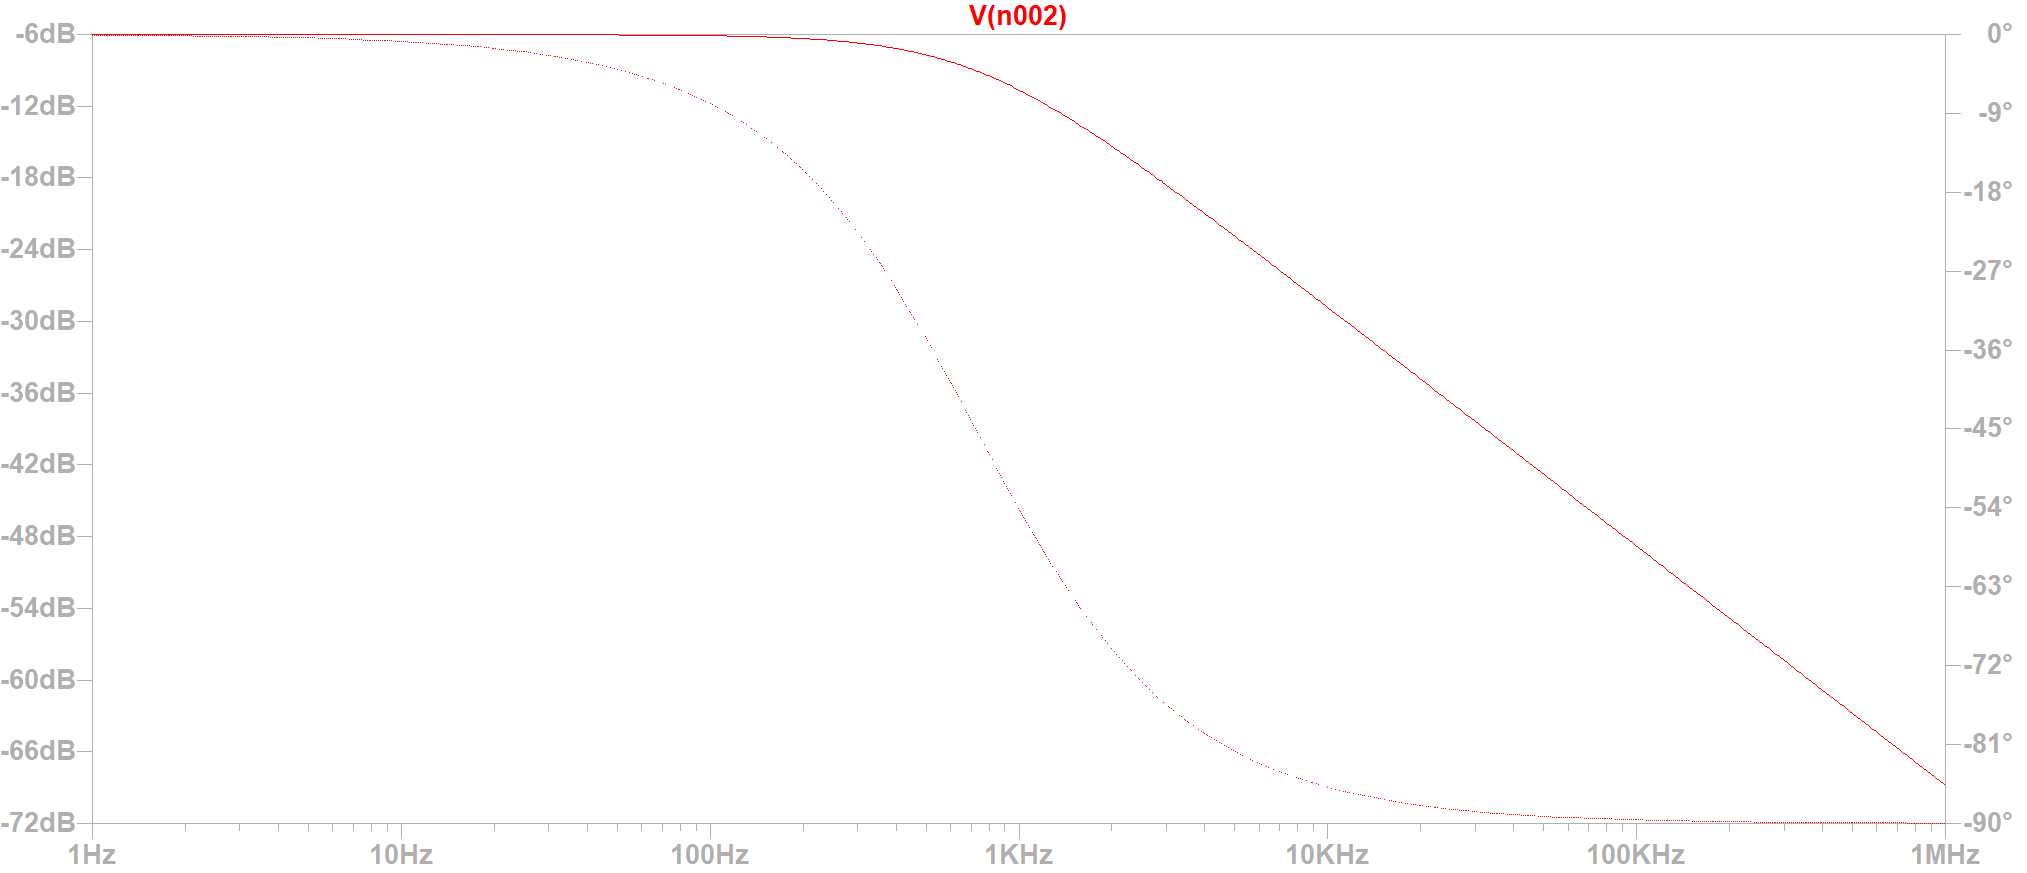
\includegraphics[width=150mm]{bode_filter01.png}
  \caption{Bode-Diagramm RC-Tiefpassfilter 1. Ordnung}
\end{figure}

\noindent Ein Bode-Diagramm dient der Darstellung der Filtereigenschaften. Auf der X-Achse wird hierfür die Frequenz in dekadischen Abständen aufgetragen und auf der Y-Achse das Übertragungsverhalte $20\log(\frac{U_a}{U_e})$ bzw. der Phasengang.

\noindent Das Übertragungsverhalten, welches als Quotient von Ausgangs- und Eingangsspannung definiert ist, ergibt sich aus folgender Formel:
\begin{figure}[H]
  \centering
  $\frac{U_a}{U_e} = \frac{Z_{C1}}{Z_{R1}+Z_{C1}} = \frac{\frac{1}{j\omega C1}}{R1+\frac{1}{j\omega C1}} = \frac{1}{1+j\omega R1C1}$
\end{figure}
Wenn die Frequenz bei 0 liegt, dann sind Aus- und Eingangsspannung gleich groß. Geht die Frequenz gegen $\infty$ lässt der Filter kein Signal mehr durch.

\noindent Die Grenzfrequenz des Filters wird bei
\begin{figure}[H]
  \centering
  $f_c = \frac{1}{2\pi R1C1} \approx 723Hz$
\end{figure}
\noindent erreicht.\\
Hier beträgt die Dämpfung ca. $-3dB$ und der Phasengang $-45^{\circ}$ und die Spannung über $R1$ und $C1$ ist gleich. Man kann anhand des Diagramms auch gut erkennen, dass die Filtersteilheit bei einem RC-Tiefpass 1.Ordnung $-20dB/Dekade$ beträgt.

\section{RL-Hochpassfilter 1. Ordnung}

\subsection{Aufgabenstellung}
Die Sprungantwort und der Amplituden- bzw. Phasengang eines RL-Hochpassfilters 1. Ordnung soll mittels LTSpice simuliert werden.

\subsection{Schaltplan}

\begin{figure}[H]
  \centering
  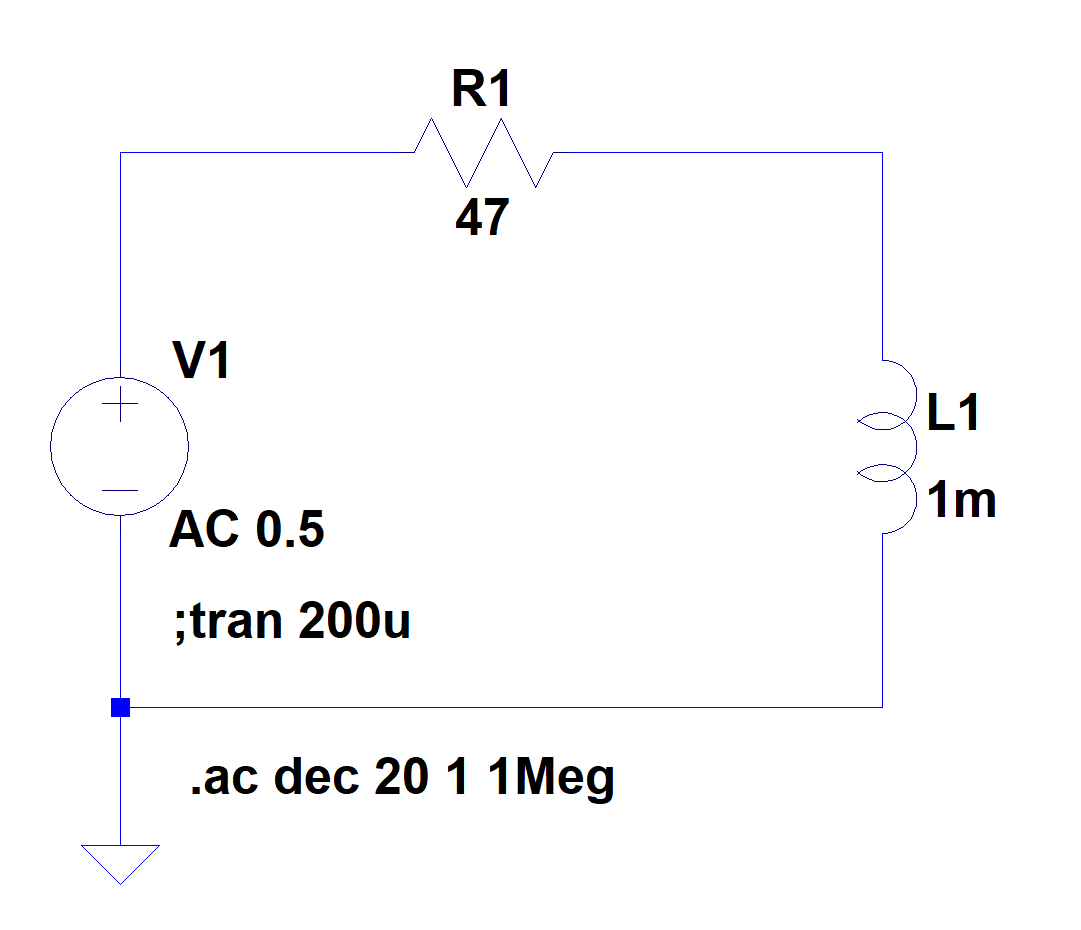
\includegraphics[width=100mm]{filter02_schaltung.PNG}
  \caption{RL-Hochpassfilter 1. Ordnung}
\end{figure}

\subsection{Durchführung}
Zuerst wird die RL-Schaltung mit $R1 = 47\Omega$, $L1 = 1mH$ und $R_L = 0 \Omega$ zusammengefügt. Dazu wird mit der PULSE-Option der Sprung von $0V$ auf $1V$ angelegt. Die Sprungantwort des Systems wird dann im Bereich von $0s$ bis $200\mu s$ geplotted. Nun soll der Amplituden- und Phasengang simuliert werden. Dazu wird eine sinusförmige Spannung mit $1V_{pp}$ ($0,5V$ Amplitude) angelegt. Es wird eine dekadische Transientensimulation im Bereich von $1Hz$ bis $1MHz$ durchgeführt und das daraus resultierende Bode-Diagramm aufgezeichnet. Danach wird der Widerstand $R_L$ auf $1,2\Omega$ geändert, die Simulation des Amplituden- und Phasenganges wiederholt und das neue Bode-Diagramm aufgezeichnet.

\subsection{Ergebnis}

\begin{figure}[H]
  \centering
  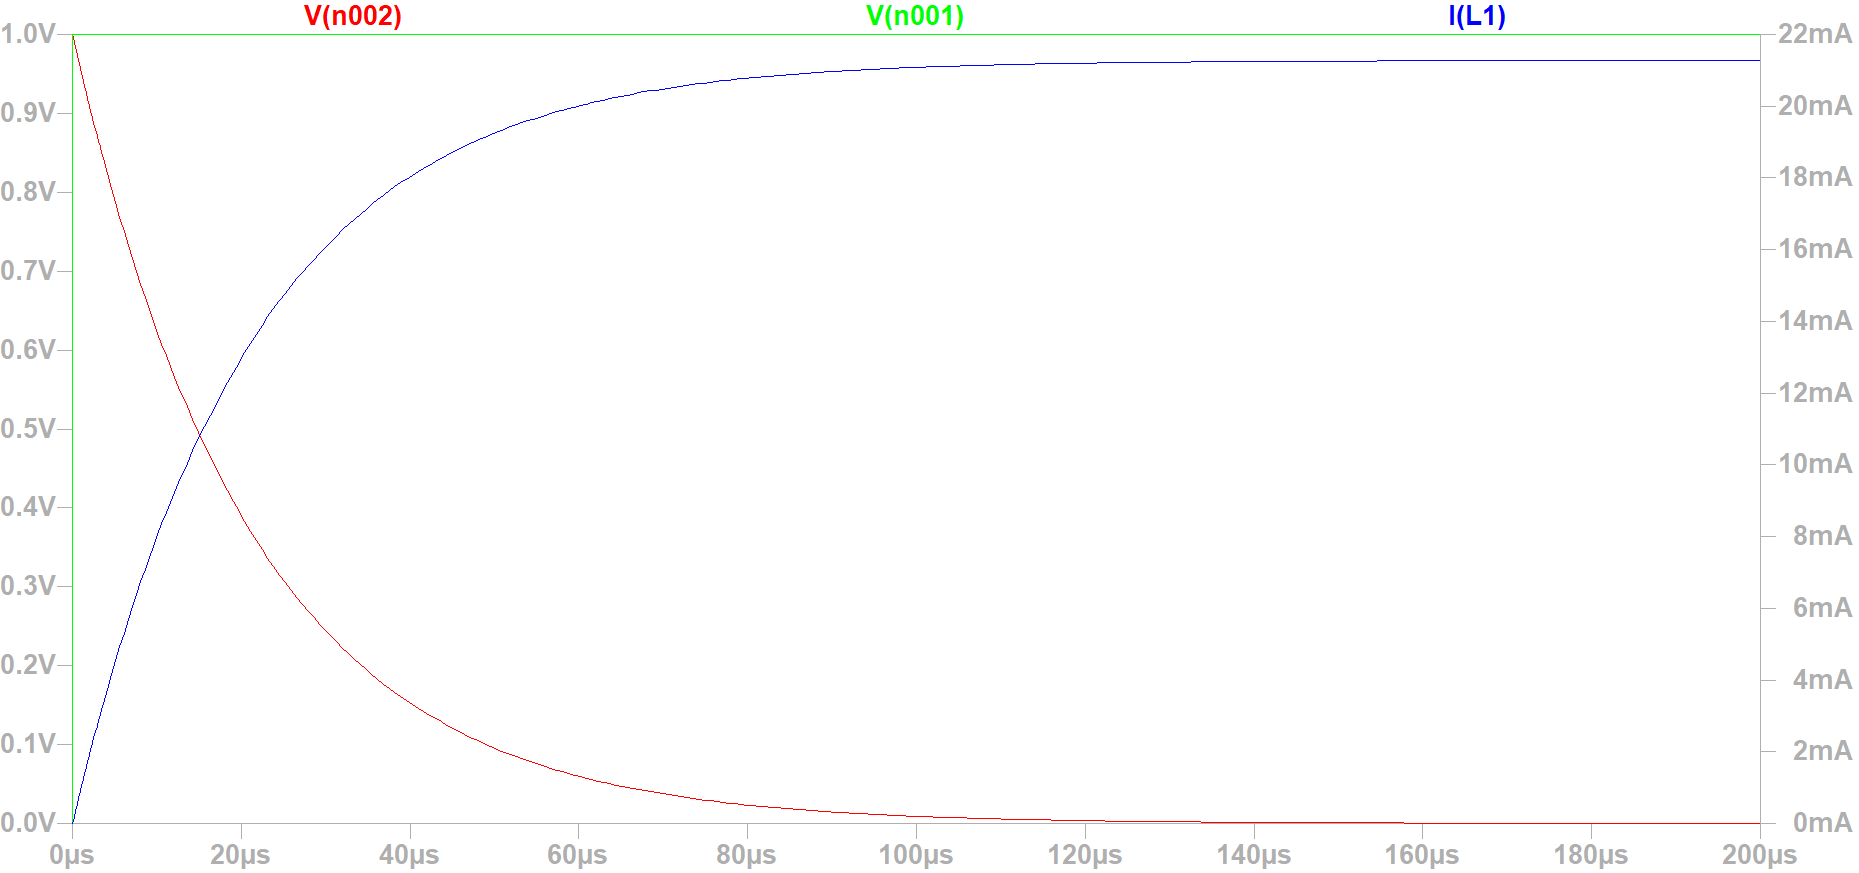
\includegraphics[width=150mm]{sprungantwort_filter02.png}
  \caption{Sprungantwort RL-Hochpassfilter 1. Ordnung}
\end{figure}

Anhand dieses Diagramms erkennt man sehr gut, wie der Strom $I(L1)$ an der Spule zuerst minimal ist und bei fallender Spannung $V(n002)$ an der Spule immer stärker ansteigt. Der Strom erreicht sein Maximum, sobald die Spannung an der Spule minimal ist.\\\\
Die Zeitkonstante
\begin{figure}[H]
  \centering
  $\tau = \frac{L1}{R1} = \frac{1mH}{47} \approx 21,3\mu s$
\end{figure}
\noindent besagt, dass $L1$ nach $21,3\mu s$ zu 63\% aufmagnetisiert ist. Nach $5*\tau \approx 106,4\mu s$ ist $L1$ zu 99\% aufmagnetisiert, der Strom is maximal.

\begin{figure}[H]
  \centering
  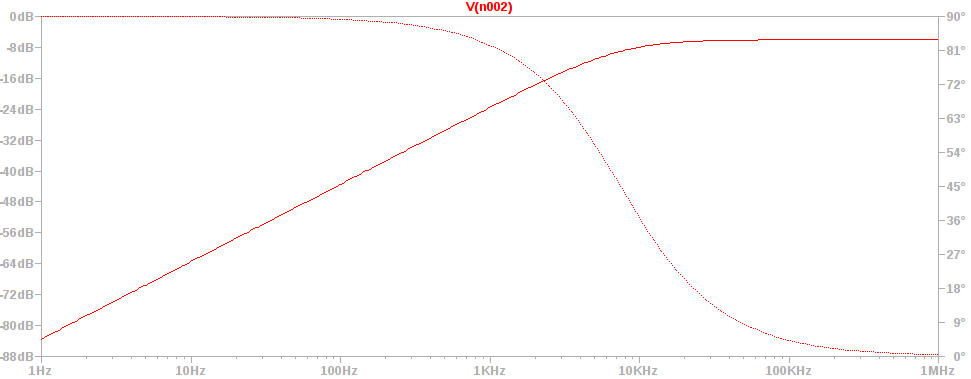
\includegraphics[width=150mm]{bode_filter02.png}
  \caption{Bode-Diagramm RL-Hochpassfilter 1. Ordnung}
\end{figure}

\noindent Das Übertragungsverhalten, welches als Quotient von Ausgangs- und Eingangsspannung definiert ist, ergibt sich aus folgender Formel:
\begin{figure}[H]
  \centering
  $\frac{U_a}{U_e} = \frac{Z_{L1}}{Z_{R1}+Z_{L1}} = \frac{j\omega L1}{R1 + j\omega L1}$
\end{figure}
Wenn die Frequenz bei 0 liegt, dann dann lässt der Filter kein Signal durch. Geht die Frequenz gegen $\infty$, dann sind Aus- und Eingangsspannung gleich groß.

\noindent Die Grenzfrequenz des Filters wird bei
\begin{figure}[H]
  \centering
  $f_c = \frac{R1}{2*\pi*L1} \approx 7,5kHz$
\end{figure}
\noindent erreicht.\\
Hier beträgt die Dämpfung ca. $3dB$ und der Phasengang $45^{\circ}$ und die Spannung über $R1$ und $L1$ ist gleich. Man kann anhand des Diagramms auch gut erkennen, dass die Filtersteilheit bei einem RL-Tiefpass 1.Ordnung $20dB/Dekade$ beträgt.

\begin{figure}[H]
  \centering
  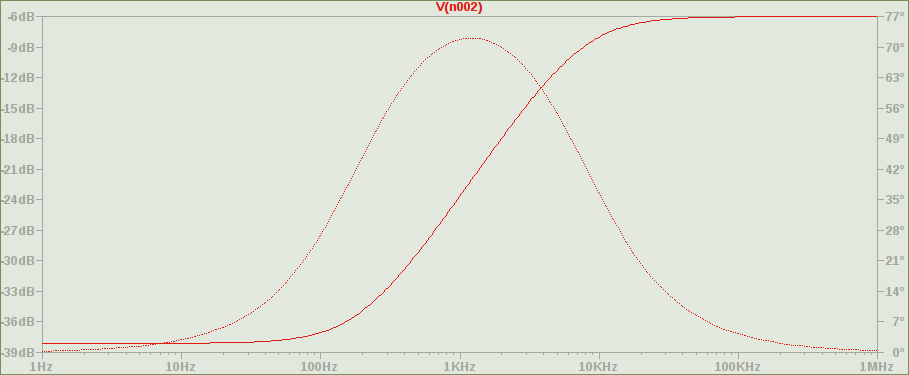
\includegraphics[width=150mm]{bode_filter02R.png}
  \caption{Bode-Diagramm RL-Hochpassfilter 1. Ordnung mit Serienwiderstand $1,2\Omega$}
\end{figure}

\noindent Durch den parasitären Serienwiderstand wird die Schaltung verändert und somit auch die Filtereigenschaften. Verglichen mit dem Bode-Diagramm für das System ohne parasitären Serienwiderstand zeigt sich, dass hier eine starke Veränderung des gewünschten Hochpassverhaltens eintritt und dieses kaum mehr vorhanden ist.

\end{document}
